\section{Method}\label{meth}
Consider a population stratified by $N_g$ patches and $N_a$ age groups.%
\footnote{We use different notation than \citet{Arenas2020};
  a comparison is given in Table~\ref{tab:notation}.}
Let $P_{ga}$ be the number of people in patch $g$ and age group $a$.
Let $y$ denote $N_y$ different types of contacts (e.g.\ household, workplace, etc.).
Let $B_{gg'}$ be the proportion of population $P_{g}$ who travel to $g'$ each day,
or the ``mobility matrix''.%
\footnote{\citet{Arenas2020} consider different mobility patterns by age: $B_{gg'a}$.
  For simplicity, we consider $B_{gg'}$ unstratified by age,
  but age stratification could be added to our approach.}
% ==================================================================================================
\subsection{Original Approach}\label{meth.orig}
\citet{Arenas2020} model the force of infection (incidence per susceptible) experienced by population $P_{ga}$ as:
\begin{equation}\label{eq:Arenas.lambda}
  \lambda_{ga}(t) = (1-\rho_a)\,\Phi_{ga}(t) + \rho_a \sum_{g^*} B_{gg^*a} \Phi_{g^*a}(t)
\end{equation}
where:
$\Phi_{ga}(t)$ is the probability of acquiring infection while in patch $g$;
and $\rho_{a} \in [0,1]$ is an age-specific overall mobility factor.
Thus, $\lambda_{ga}(t)$ is the sum of infection probabilities
from the residence patch $g$, and from visited patches $g^* \ne g$.
The probability $\Phi_{g^*a}(t)$ is modelled using
the chained binomial for multiple exposures \cite{Kaplan1990}:
\begin{equation}\label{eq:Arenas.Phi}
  \Phi_{g^*a}(t) = 1 - \prod_{a'}\prod_{g'} \prod_{i'} {\left(1 - \beta_{i'}\right)}
    ^{\,f_{g^*}C_a\,\theta_{aa'} \Omega_{g^*g'i'a'}}
\end{equation}
where:
$\beta_i$ is the per-contact transmission probability associated with infectious state $i$;
$f_{g^*}$ is a density factor associated with patch $g^*$;
$C_a$ is the expected number of contacts made per person per day in age group $a$;
$\theta_{aa'}$ is the age distribution of those contacts, derived from \cite{Prem2017} for Spain,
such that $\sum_{a'} \theta_{aa'} = 1$;
and $\Omega_{g^*g'i'a'}$ is the proportion of individuals present in patch $g^*$
who reside in patch $g'$ and who are in infectious state $i'$, for each age group $a'$.
This proportion $\Omega_{g^*g'i'a'}$ is defined as:
\begin{equation}\label{eq:Arenas.Omega}
  \Omega_{g^*g'a'i'} = \frac{P_{g'i'a'} M_{g'g^*a'}}{\sum_{g'i'} P_{g'i'a'} M_{g'g^*a'}}
\end{equation}
where $M_{gg'a}$ is a convenience simplification of the mobility matrix:
\begin{equation}\label{eq:Arenas.M}
  M_{gg'a} = (1-\rho_a)\,\delta_{gg'} + \rho_a B_{gg'a}
\end{equation}
\par
This model of infection captures important mixing patterns related to recurrent mobility
that are relevant to epidemic modelling on relatively small spatial and time scales.
However, the model could be improved by
separating different contact types throughout the force of infection equation,
and by allowing age mixing patterns to respond to local demographic and intervention conditions.
Three specific issues with the original approach are as follows:
\begin{enumerate}
  \item \textbf{Contact balancing:}\label{issue:balance}
  % SM: an assumption here is also that infection-attributable death
  %     does not alter the age-distribution, or mixing, so could speak to that as well?
  %     or perhaps in discussion section? i.e. like we do with HIV for example where
  %     we explicitly account for HIV-attributable death reducing a group's available contacts
  %     (b/c less people over time)
  % JK: @SM added to the conclusion! (end of para 2)
  % SM: noted and nice!
  The contact balancing principle states that
  the total number of contacts formed by group $a$ with group $a'$
  should equal the number formed by group $a'$ with group $a$ \cite{Arregui2018}:
  \begin{equation}\label{eq:balance}
    P_{a} C_{a} \theta_{aa'} = P_{a'} C_{a'} \theta_{a'a}
  \end{equation}
  For a model with non-random age mixing and random (proportionate) mixing by patches,
  % SM: do we mean random or proportionate here?
  % JK: @SM Reflecting on it, I personally perceive these words as interchangeable regarding mixing,
  %     since I think a "correct" implementation of "random" mixing would be proportionate
  %     to the total contacts made available by each group (pop size * #-contacts per-person),
  %     and for this reason I prefer "random", as I think it is a slightly more accessible word
  %     (readers unfamiliar with mixing may wonder: "proportionate" to what? --
  %     and we could explain/define but then it may detract from the flow of ideas)
  %     For now, what about "random (proportionate)" as edited above?
  % SM: agree but its just that in the ID modeling textbooks
  %     (and in how we teach about mixing and balancing partnerships)
  %     though, random is different than proportioante mixing.
  %     i.e. random does not account for subgroup population size
  %     (i.e. does not have to account for how many contacts could be on offer).
  %     Its ok as long as clearly defined....i.e. would consider that other modelers
  %     (esp HIV/STI modelers) would read this the way I have and expect it to have been proportionate
  %     so I like the solution you posed by explicitly defining that when you uset he term 'random' here
  %     - you are referring to propotionate to the total contacts made available by each group.
  Eq.~(\ref{eq:balance}) could be satisfied by a single fixed age mixing matrix $\theta_{aa'}$,
  i.e. for the population overall.
  However, in the context of patch-based mixing reflecting recurrent mobility,
  Eq.~(\ref{eq:balance}) should be satisfied in each mixing context (patch).
  Specifically, if different patches have different age distributions,
  or different rates of per-person contact formation due to household size, employment, etc.,
  then it would not be possible to satisfy Eq.~(\ref{eq:balance})
  with a single fixed age mixing matrix $\theta_{aa'}$.
  % JK: added the edits above
  The implications of violating Eq.~(\ref{eq:balance}) depend on
  relative differences in demographics and/or contact rates by patch and/or age group.
  For example, if a given patch skews younger than average in age,
  and most contacts are formed with other members of the same patch,
  then fixed average $\theta_{aa'}$ would
  underestimate the number of younger contacts among residents of this patch,
  and overestimate the number of older contacts.
  % SM: in which patch would that occur, or would it be overall (sum of patches)?
  % JK: I changed the example to hopefully be more clear
  \item \textbf{Age mixing by contact type:}\label{issue:age-mix}
  A related issue is that the expected contact rates by age group $C_a$ reflect
  the summation of different types of contacts,
  and so the fixed age mixing matrix $\theta_{aa'}$ is applied to all contact types.
  As such, changes to the numbers of each type of contact
  are not paired with changes the overall mixing patterns.
  % SM: so saying here that overall reductions in contact rates due to an intervention
  %     subsume the effect of the intervention across contact types?
  % JK: Yep!
  As illustrated by the \polymod study \cite{Mossong2008}, age mixing patterns vary by contact type,
  such as highly age-assortative mixing in schools.
  Thus, differential reductions in each contact type would affect overall age mixing patterns.
  For example, if reductions in school-related contacts due to school closures
  were not reflected in $\theta_{aa'}$,
  then the relative contribution of children to overall transmission
  could be overestimated during the period of school closures.
  % SM: so here the example is with age-specific effects of the intervention vs. by type of contacts?
  %     clarify this a bit more re: the key message/point here in the example....
  %     do we mean reduced non-household contacts between working-aged adults?
  % JK: @SM hopefully the revisions & example above now flow better?
  % SM: yes
  \item \textbf{Modelling contact \& mobility reductions:}\label{issue:mobility}
  The term $(1-\rho_a)\,\Phi_{ga}(t)$ in Eq.~(\ref{eq:Arenas.lambda})
  represents transmission to non-mobile individuals in patch $g$.
  The associated definitions in Eqs.~(\ref{eq:Arenas.Phi}--\ref{eq:Arenas.M})
  consider transmission to these non-mobile individuals from visitors to patch $g$.
  Such definitions therefore imply that
  non-mobile individuals still form contacts with visitors to their residence patch.
  However, it may be useful to model some or all non-mobile individuals
  as only forming contacts with other individuals from their residence patch.
  That is, scenarios may exist wherein a fraction of the population only has
  household contacts, as could be the case with public health measures such as lockdowns.
  % MH: This section is quite unclear.
  %     Not sure I follow logic on why proportional reductions in mobility and non-home contacts
  %     would suggest non-mobile individuals are forming home contacts with mobile visitors?
  % JK: Sorry its unclear - what I meant to say is that
  %     proportional reductions in mobility and non-home contacts
  %     would suggest non-mobile individuals are forming *only home contacts*,
  %     which *shouldn't* be formed with mobile visitors, but that's what the model does, so it's kinda "wrong".
  %     Have revised entirely to re-frame it hopefully in a more simple way.
  As illustrated in Figure~\ref{fig:nm}, the original approach may
  overestimate inter-patch connectivity during periods of reduced mobility (via lockdowns)
  versus an approach in which some or all non-mobile populations are limited to
  contacts with others from their residence patch and not with visitors.
  Thus, the original approach \cite{Arenas2020} could underestimate
  the impact of confinement lockdown strategies on inter-patch transmission reduction.
  % SM: impact on trasmission reduction or transmission?
  % JK: Ah yes, transmission reduction -- good catch!
  % SM: not sure the following sentence is needed.
  % JK: Sounds good -- will remove it!
  %     While it may be desirable to sometimes allow mixing of ``non-mobile'' individuals
  %     with visitors to their residence patch,
  %     the original approach does not provide a parameterization to prevent this from happening.
\end{enumerate}
We therefore develop a refinement of the original approach,
with the aim of addressing the above three issues.
% ==================================================================================================
\subsection{Proposed Approach}\label{meth.prop}
In the proposed approach, the contributions of different contact types to the force of infection
are added to the binomial function for multiple exposures:
\begin{equation}
  \lambda_{ga}(t) = 1 - \prod_{y}\prod_{g'}\prod_{a'}\prod_{i'} {\left(1 - \beta_{i'}\right)}
  ^{C_{gag'a'y} \Omega_{g'a'i'}}
\end{equation}
where:
$C_{gag'a'y}$ is the expected number of type $y$ contacts formed per person per day
among individuals in population $P_{ga}$ with those in population $P_{g'a'}$;
and $\Omega_{g'a'i'}$ is the proportion of individuals in residing in patch $g'$ and age group $a'$
who are in infectious state $i'$:
\begin{equation}
  \Omega_{g'a'i'} = \frac{P_{g'a'i'}}{P_{g'a'}}
\end{equation}
For each type of contact, $C_{gag'a'y}$ is defined to reflect
both age-related and mobility-related mixing factors,
as described in the following subsections.
To support these descriptions, we will refer to Figures from an example application,
although the details of the application and the Figures are given in \S~\ref{ex}.
Collecting the full network of contacts in the matrix $C_{gag'a'y}$
provides a representation that is easy to interpret,
% MH: unsure about use of parsimonious here??   collecting full network of contacts is frugal?
% JK: Aha, I meant like the "principle of parsimony", although I guess it is not reading right...
%     Like, rather than have the mixing equation split up into 3+ different variables,
%     collecting all the contacts into one big matrix means that the whole thing we care about
%     is "all in one place", and it kinda helps us interpret it.
%     IDK, maybe can just skip to "allows us to ..." below if the above edit doesn't help.
and allows us to compute various properties, like the margins in $a,a'$ or $g,g'$,
and whether contact balancing is satisfied per Eq.~(\ref{eq:balance}).
Additionally, separating contact types allows the incorporation of
different probabilities of transmission per contact type $\beta_{i'y}$, if desired.
% --------------------------------------------------------------------------------------------------
\subsubsection{Age Mixing}\label{meth.prop.mix.age}
\citet{Prem2021} project contact patterns by 5-year age groups
from the \polymod study \cite{Mossong2008} onto 177 countries,
considering various demographic data.
These contact matrices represent $C_{aa'y}$:
the expected number of type $y$ contacts formed per day among
individuals in age group $a$ with those in age group $a'$.
Four types of contact are considered: ``home'', ``work'', ``school'', and ``others''%
\footnote{The ``others'' contact type in \cite{Prem2021} is itself derived from
  the combination of ``leisure'', ``transport'', and ``other'' contact types from \cite{Mossong2008},
  while the ``home'', ``work'', and ``school'' types are the same between the studies.}
(Figure~\ref{fig:C4AAy0}).
We aim to incorporate these contact numbers and patterns into $C_{gag'a'y}$.
% HM: do we need describe polymod data in Data section as it s Canada specific?
% JK: good point -- I think we have not mentioned that it is Canada specific there, but I've added now.
\par
The first challenge is that the contact matrices $C_{aa'y}$ are
inherently weighted by the underlying population age distribution---%
the proportion of expected contacts with age group~$a'$ is proportional to the size of age group~$a'$.
To overcome this challenge and apply these patterns to new population age structures,
\citet{Arregui2018} suggest to divide by the population age distribution
to obtain an ``unweighted'' matrix $C^u_{aa'y}$ (Figure~\ref{fig:C4AAy1}):%
\footnote{The matrix $C^u_{aa'y}$ could also be interpreted as
  the expected contact matrix for a population with a rectangular demographic pyramid \cite{Arregui2018}.}
\begin{equation}\label{eq:C^u}
  C^u_{aa'y} = C_{aa'y} \frac{\bar{P}}{P_{a'}}
\end{equation}
where $\bar{P}$ is the mean of $P_{a'}$.
\par
The next challenge is that $C^u_{aa'y}$ may not satisfy
the contact balancing principle, Eq.~(\ref{eq:balance}),
due to sampling and/or reporting error in the \polymod survey.
% SM: did not understand what was meant by "...vs that of the contacts the respondents reported."
%     refphrase for clarity
% JK: @SM (re. above) better?
% SM: yes
To ensure that the overall mixing matrix $C_{gag'a'y}$ will satisfy the balancing principle,
the input age mixing matrix $C^u_{aa'y}$ must satisfy the principle.
% SM: rephrase sentence for clarity as sentence circular?
% JK: @SM better? -- added "overall" vs "input" as C_gagay is derived from C_aay
A simple solution is to average $C^u_{aa'y}$ with its transpose
to obtain the ``balanced'' matrix $C^{ub}_{aa'y}$ (Figure~\ref{fig:C4AAy2}):
\begin{equation}\label{eq:C^ub}
  C^{ub}_{aa'y} = \frac{1}{2}\left[C^u_{aa'y} + {C^u_{aa'y}}^{T}\right]
\end{equation}
This operation may change the margin $C_{ay}$, representing
the total type $y$ contacts formed by individuals in age group $a$.
However, such changes are reasonable if understood as a correction for sampling bias.%
\footnote{A perfect survey in a closed population would produce
  a contact matrix $C^u_{aa'y}$ that is already balanced.}
\par
A final challenge in applying the contact matrices from \cite{Prem2021} is that
% SM: love this part and the solution!
% JK: @SM :) "it was easy". Narrator: it was not.
% SM: LOL!
the 5-year age groups may not align with the age groups of interest.
Overcoming this challenge is not theoretically required to obtain $C_{gag'a'y}$,
but we describe a solution here in case it is useful for modelling applications.
We begin by upsampling the contact matrix from 5-year age groups $a_5$ to 1-year age groups $a_1$
using bilinear interpolation, based on the midpoints of each age group,
and scaled by a factor of $1/5$.
To avoid edge effects associated with many interpolation implementations,
we first pad the matrix by replicating the edges diagonally.
If the desired age groups extend beyond the maximum age group of 80 available in \cite{Prem2021},
diagonal padding can also be used to approximate the trends in the additional age groups.
Then, given the age groups of interest $a_*$ (which may have irregular widths),
we aggregate $C^{ub}_{a_1a'_1y}$ to obtain $C^{ub}_{a_*a'_*y}$
using matrix multiplication with indicator matrix $A$:
\begin{equation}\label{eq:Ca*}
  C^{ub}_{a_*a'_*y} = \frac{A_{a_*a_1}}{\sum_{a_1} A_{a_*a_1}} C^{ub}_{a_1a'_1y} A_{a'_*a'_1}^T,\qquad
  A_{a_*a_1} = \begin{cases}
    1, & a_1 \in a_* \\
    0, & a_1 \not\in a_* \\
  \end{cases}
\end{equation}
The right-hand $A^T$ term \textit{sums} the total number of contacts
formed with the 1-year ``other'' age groups $a'_1$ corresponding to $a'_*$.
The left-hand $A$ term \textit{averages} the total number of contacts
formed from the 1-year ``self'' age groups $a_1$ corresponding to $a_*$.
The average weights each 1-year age group $a_1$ equally,
although other weights could be incorporated through the nonzero values of $A$.
Another interpretation of the normalization sum is the widths of the age groups $a_*$.
\par
The resulting matrix $C^{ub}_{a_*a'_*y}$ represents the expected contacts among age groups $a_*$
when mixing with a population having equal proportion in all age groups $a'_*$ (regardless of their width).
Thus, $C^{ub}_{a_*a'_*y}$ can later be multiplied by the population age distribution of interest%
---reversing Equation~(\ref{eq:C^u})---%
to obtain the expected number of contacts when mixing with that population.
This approach then addresses issues \ref{issue:balance}~and~\ref{issue:age-mix}
described in \S~\ref{meth.orig}.
% --------------------------------------------------------------------------------------------------
\subsubsection{Mobility-Related Mixing}\label{meth.prop.mix.mob}
% MH: Found the concept of home vs. traveling pools and mobile vs. not mobile individuals confusing upon first read.
%     Have made some suggestions to improve clarity.
% JK: Thanks! As you can see, I did a bit of an overhaul using more definitions.
%     Hopefully it's better now?
% SM: read well and flowed nicely
In conceptualizing mobility-related mixing,
we define two types of contexts in which contacts can be formed:
\begin{itemize}
  \item \textbf{Home pools:} where contacts are formed exclusively with
  other residents of the same patch (e.g. for household contacts)
  \item \textbf{Travel pools:} where contacts are formed with
  individuals from any patch who are present in the pool (e.g. for work contacts)
\end{itemize}
We model one home pool and one travel pool associated with each patch,
as illustrated in Figure~\ref{fig:pools}.
\begin{figure}
  \centering
  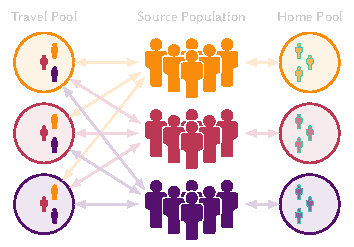
\includegraphics[width=.6\linewidth]{pools-half-home}
  \caption{Toy example of ``home'' vs ``travel'' mixing pools
    for a network with 3 patches and 50\% individuals mobile.
    Contacts in the home pool are formed exclusively with other members of the residence patch,
    whereas contacts in the travel pool may be formed with any visitors to the patch}
  \label{fig:pools}
  \floatfoot{Non-mobile populations are indicated with faded colour and green outline}
\end{figure}
\par
In this conceptualization, only contacts associated with travel pools are influenced by
the population mobility matrix $B_{gg'}$,
representing the expected proportions of individuals from patch $g$ who visit patch $g'$ per day.
For contacts associated with home pools, this matrix is functionally replaced with
an identity matrix $\delta_{gg'}$.
It is not necessary to assume that
all contacts of any particular type are formed in only one type of pool.
Rather, we introduce a parameter $h_y \in [0,1]$ representing
the proportion of type $y$ contacts that are formed in the home pool,
and the remainder ($1-h_y$) are formed with travel pools.
For example, we could have
$h_y = 1$ for household contacts, $h_y = 0$ for work contacts, and $h_y = 0.5$ for school contacts.
Thus, the expected contacts formed by individuals in patch $g$ are distributed across three situations:
\begin{enumerate}
  \item \textbf{Mobile Away:}\label{situ:mob-away}
  individual travelled from patch $g$ to patch $g'$ and formed contacts within travel pool $g'$\\
  Proportion of contacts: $(1-h_y) B_{gg' \, (g \ne g')}$
  \item \textbf{Mobile at Home:}\label{situ:mob-at-home}
  individual formed contacts within their local travel pool $g$\\
  Proportion of contacts: $(1-h_y) B_{gg' \, (g = g')}$
  \item \textbf{Non-Mobile at Home:}\label{situ:non-mob}
  individual formed contacts within their local home pool $g$\\
  Proportion of contacts: $h_y \delta_{gg'}$
\end{enumerate}
The idea of ``home pools'' is new versus \cite{Arenas2020},
and allows us to address issue~\ref{issue:mobility}
by introducing situation~\ref{situ:non-mob}.
Thus in \cite{Arenas2020}, all mixing was implicitly modelled using ``travel pools'',
and individuals described as ``non-mobile'' reflected situation~\ref{situ:mob-at-home}.
\par
In the context of reduced mobility, we do not assume that rows of $B_{gg'}$ sum to~1.
The ``missing'' proportion $1 - \sum_{g'} B_{gg'}$ is then taken to represent
non-mobile individuals, who do not form any mobility-related contacts
(situations \ref{situ:mob-away}~and~\ref{situ:mob-at-home}) that day.
In \S~\ref{app.mob} we discuss some details about
generating a mobility matrix $B_{gg'}$ with these properties, based on mobile phone data.
% MH: Would save this comment until the end of the section on mobility-related mixing
% JK: How is here now?
\par
To calculate $C_{gag'a'y}$ using these assumptions,
we begin by considering the travel pool in patch $g^*$.
The effective number of individuals from population $P_{ga}$
who are present in the pool is given by:%
\footnote{If residents of different patches might have relatively different numbers of contacts,
  a scaling factor could be applied here.}
\begin{equation}\label{eq:P*}
  P^{\,g^*}_{gay} = (1-h_y) B_{gg^*} P_{ga}
\end{equation}
There is no distinction between situations \ref{situ:mob-away}~and~\ref{situ:mob-at-home}
in Eq.~(\ref{eq:P*}),
as both are already reflected in the off-diagonal and diagonal elements of $B_{gg'}$, respectively.
If we assume that mixing by residence patch $g$ within the pool is random,
we need only consider age mixing within the pool.
Under completely random mixing,
% SM: do we mean proportionate mixing?
% JK: see comment above about "random" vs "proportionate"
the total number of contacts formed between $P^{\,g^*}_{gay}$ and $P^{\,g^*}_{g'a'y}$
is given by the outer product:
\begin{equation}\label{eq:X*r.gagay}
  X^{g^*r}_{gag'a'y} = P^{\,g^*}_{gay} \otimes
    \left. P^{\,g^*}_{g'a'y} \middle/ \textstyle\sum_{g'a'} P^{\,g^*}_{g'a'y}\right.
\end{equation}
where the first term represents the absolute population size of ``self'',
and the second term represents proportions of their contacts among ``other'' strata.
Then, the patterns of age mixing can be applied via multiplication:
\begin{equation}\label{eq:X*.gagay}
  X^{g^*}_{gag'a'y} = X^{g^*r}_{gag'a'y}
    \left.C^{ub}_{aa'y} \middle/ \textstyle\sum_{a'_1} A_{a'a'_1}\right.
\end{equation}
since $X^{g^*r}_{gag'a'y}$ is proportional to the population age distribution of ``others'',
and will therefore act to reverse Eq.~(\ref{eq:C^u}) as planned.
The term $\sum_{a'_1} A_{a'a'_1}$ is from Eq.~(\ref{eq:Ca*}),
representing the widths of the age groups $a'$.
It is necessary to divide by the widths of age groups $a'$ since
both $X^{g^*r}_{gag'a'y}$ and $C^{ub}_{aa'y}$ are proportional to these widths,
but the proportionality should only be singular overall.
We could have applied this normalization to $C^{ub}_{aa'y}$
in Eq.~(\ref{eq:Ca*}) in the same way as for $a$,
but this would make $C^{ub}_{aa'y}$ harder to interpret,
as it would no longer represent the expected numbers of contacts for each age group.
\par
Mixing within home pools (situation~\ref{situ:non-mob})
can be modelled similar to mixing within travel pools,
with one small modification: replacing $(1-h_y) B_{gg'}$ with $h_y \delta_{gg'}$.
Following through Eqs.~(\ref{eq:P*}--\ref{eq:X*r.gagay}), we obtain $X^{h}_{gag'a'y}$,
representing the total contacts formed within home pools.
Then, the total type $y$ contacts formed between populations $P_{ga}$ and $P_{g'a'}$
across all relevant mixing pools is given by the sum:
\begin{equation}\label{eq:Xgagay}
  X_{gag'a'y} = X^h_{gag'a'y} + \sum_{g^*} X^{g^*}_{gag'a'y}
\end{equation}
It may be tempting to simplify the model for home pool contacts by
updating the mobility matrix $B_{gg'}$ similar to Eq.~(\ref{eq:Arenas.M}) from \cite{Arenas2020},
with $h_y = (1-\rho_a)$.
However, such an approach does not produce the same result as Eq.~(\ref{eq:Xgagay}),
and indeed underpins issue \ref{issue:mobility} described in \S~\ref{meth.orig}
regarding mixing of non-mobile individuals with mobile visitors to their patch.
On the other hand, if the interpretation of ``non-mobile'' is intended to allow mixing with visitors,
then $B_{gg'}$ can still be adjusted per Eq.~(\ref{eq:Arenas.M}) to simulate this behaviour.
Another implication of our approach is that
non-mobile individuals will not form mobility-related contacts.
Thus, if $\sum_{g'} B_{gg'}$ is reduced,
the total contacts formed by residents of patch $g$ would be reduced proportionately,
and changes to mixing patterns by age and patch reflected automatically.
\par
Finally, the number of type $y$ contacts formed \textit{per person}
in population $P_{ga}$ with population $P_{g'a'}$ can be obtained by
dividing $X_{gag'a'y}$ by the population size:
\begin{equation}\label{eq:Cgagay}
  C_{gag'a'y} = \frac{X_{gag'a'y}}{P_{ga}}
\end{equation}